\section{Effective Resistance \& Destination Tickets}

\begin{figure*}[!ht]
\centering
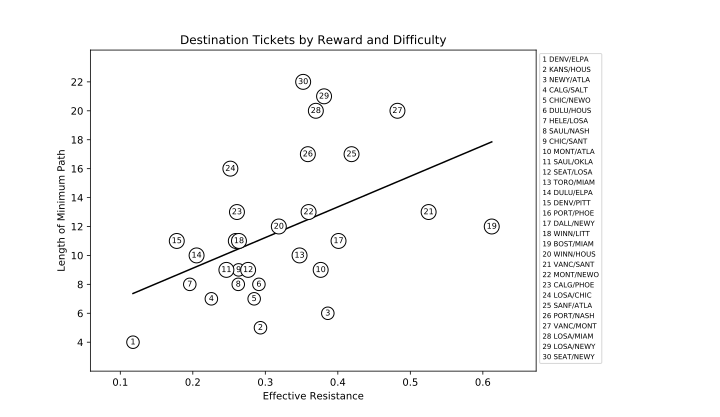
\includegraphics[scale=.8]{figures/resistance}
\caption{Destination Tickets by their effective
resistance and minimum path length.
The line of best fit gives an approximation of the
Destination Tickets that are better than average (above the line)
and worse than average (below the line) in terms
of the point value per difficulty.
Note: the $16^{th}$ Destination Ticket Portland/Phoenix is obscured
by the $18^{th}$.}
\label{fig:resistance}
\end{figure*}

\subsection{Simulations}

\begin{figure*}[!ht]
\centering
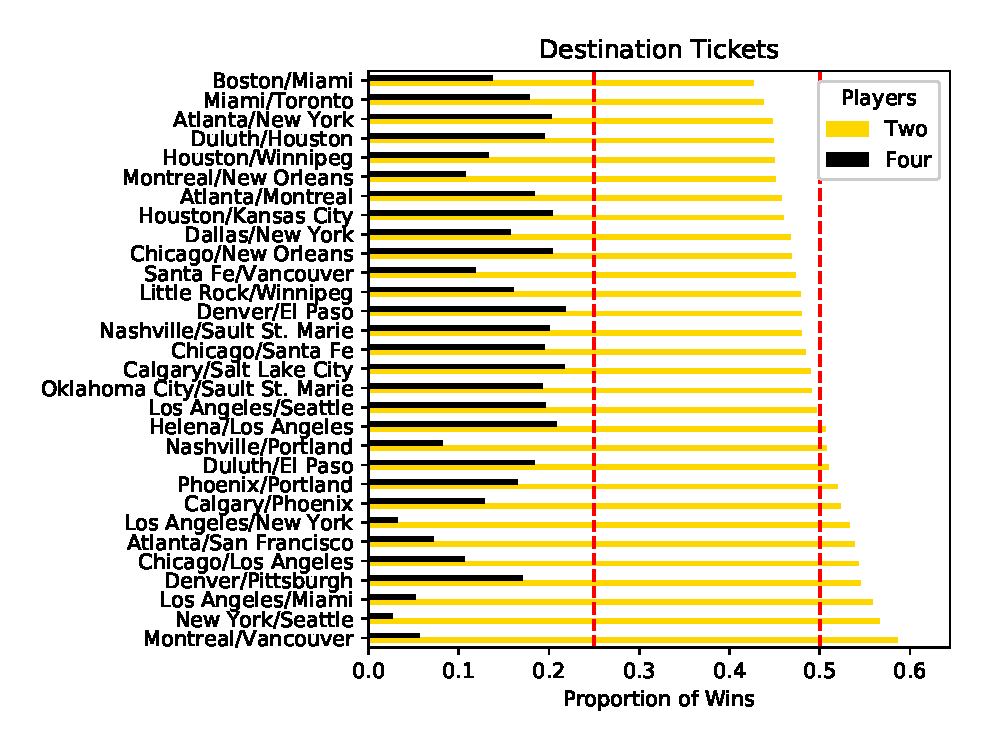
\includegraphics[scale=.8]{figures/destination_tickets}
\caption{The proportion of times that a player with a certain
Destination Ticket in their hand won.
The vertical red lines at $x=1/4$ and $x=1/2$ represent
the expected proportion of times a player with a certain Destination Ticket
would win if there was no affect. (Computed from 1000 simulations.)}
\label{fig:tickets}
\end{figure*}


%\begin{figure*}[!ht]
%\centering
%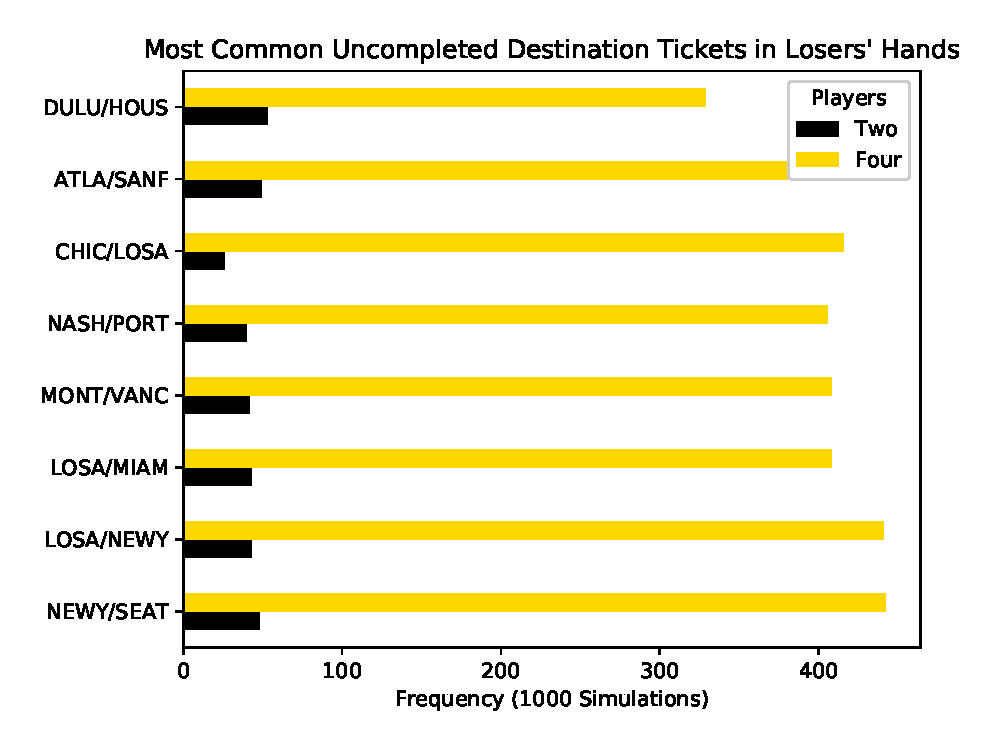
\includegraphics[scale=.8]{figures/uncompleted}
%\caption{The most common uncompleted
%Destination Tickets in the losers'
%hands at the end of 1000 simulated games.
%The disparity between two and four player
%games originates from the different number
%of losers: most of the time there are three 
%losers in the four person game whereas there is 
%always only one loser in the two person game.
%(Games were simulated using
%Silva et al.'s code.)}
%\label{fig:uncompleted}
%\end{figure*}
%
%\begin{figure*}[!ht]
%\centering
%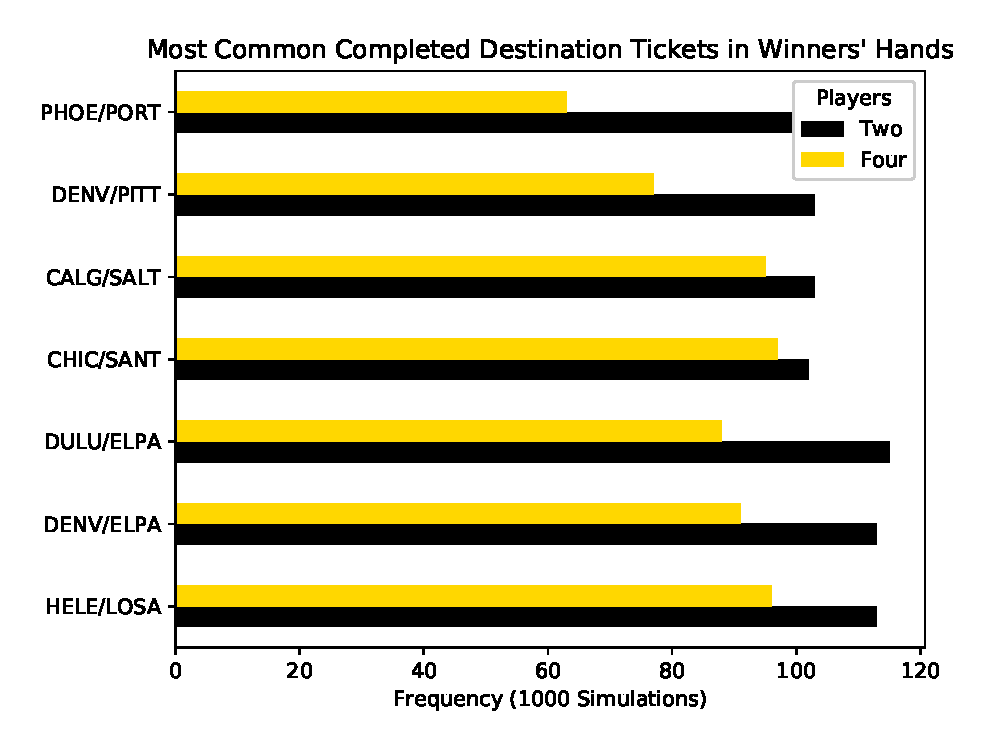
\includegraphics[scale=.8]{figures/completed}
%\caption{The most common completed
%Destination Tickets in the winners'
%hands at the end of 1000 simulated games.
%(Games were simulated using Silva et al.'s code.)}
%\label{fig:completed}
%\end{figure*}